% Draft Version 1 - Date 16/06/2020
% Draft Version 2 - Date 06/08/2020
% Draft Version 3 - Date 27/08/2020
% Draft Version 4 - Date 23/09/2020
% Draft Version 5 - Date 14/12/2020

\chapter{\titlech}\label{chap-ch}

\section{Introduction}
Every material found in nature has heterogeneity involved at different scales of length. This heterogeneity results in complex behavior leading to a significant impact on the material properties and the inherent response to different loading conditions. The prediction of the behavior due to these spatial variations in the material can be directly computed using direct numerical simulation of the finite element discretization of the heterogeneity. But any such approach needs to ensure that the mesh size is comparatively smaller than the size of the heterogeneity, leading to significant computational cost due to the enormous number of degrees of freedom. However, this does not negate the importance of taking into consideration the various high accuracy geometry development tools to study complex material structures in high performance applications.

Homogenization techniques have traditionally been used to extract effective macroscopic properties of such heterogeneous media. Semi analytical methods such as mean field homogenization (MFH) based on Eshelby tensor\cite{pierardMeanfieldHomogenizationMultiphase2004}, 
%asymptomatic homogenization theory\cite{bensoussanAsymptoticAnalysisPeriodic2011}, Bloch wave homogenization\cite{allaireComparisonTwoscaleAsymptotic2016}, 
among others, are usually restricted to simple microscopic geometries and simple material models, often under the assumption of small strains. The concept of a unit cell to determine the homogenized material properties by fitting the detailed modeling of the unit cell on macroscopic phenomenological equations was developed in \cite{hillElasticPropertiesReinforced1963} and was used to display the effectiveness of such unit cells in various studies\cite{christmanExperimentalNumericalStudy1989,tvergaardMechanicalModellingDuctile1991,baoImprovedTn7basedSystem1991,brockenbroughDeformationMetalmatrixComposites1991}. The extension of the unit cell to a history dependent constitutive behavior through micro-macro behavior can be obtained in an efficient manner by assigning a unit cell to each integration point of the macro-mesh\cite{smitPredictionMechanicalBehavior1998} and this procedure can be called homogenization based multi-scale analysis.

Multi-scale and homogenization techniques have been used to predict the collective multi-phase response of materials on the basis of the understanding of single phases and complex interfaces in materials along with the taking into account of large deformations, damage, cracking and phase transformations among other mechanical effects \cite{geersMultiscaleComputationalHomogenization2010}. Among these, computational homogenization is probably one of the most accurate techniques in upscaling the non-linear behavior of well characterized micro-structure. In this method, a computational boundary value problem (BVP) is constructed which is then numerically solved to determine the local governing behavior at the macro scale. A fully nested solution of BVP at each scale is obtained if the macro scale BVP is solved simultaneously (Figure \ref{fig-ch-homogenization}). For a  periodic micro-structure, a unit cell can be used to define the micro BVP, while a Representative Volume Element (RVE) has to be used for non-periodic ones. In the latter case, it is necessary to ensure that the RVE size is large enough to represent statistically the pertinent information of the micro-structure. Considering that larger RVEs will result in higher computation times, the critical size of the RVE needs to determined taking into account efficiency and accuracy\cite{ostoja-starzewskiMechanicsRandomMaterials2001,kanitDeterminationSizeRepresentative2003}. It is also necessary to note that a volume element becomes a true RVE only when the effective constitutive response is independent with respect to the boundary conditions that are energetically consistent, which can be satisfied by the Hill-Mandel principle.

\begin{figure}
	\centering
	\begin{subfigure}[t]{0.75\textwidth}
		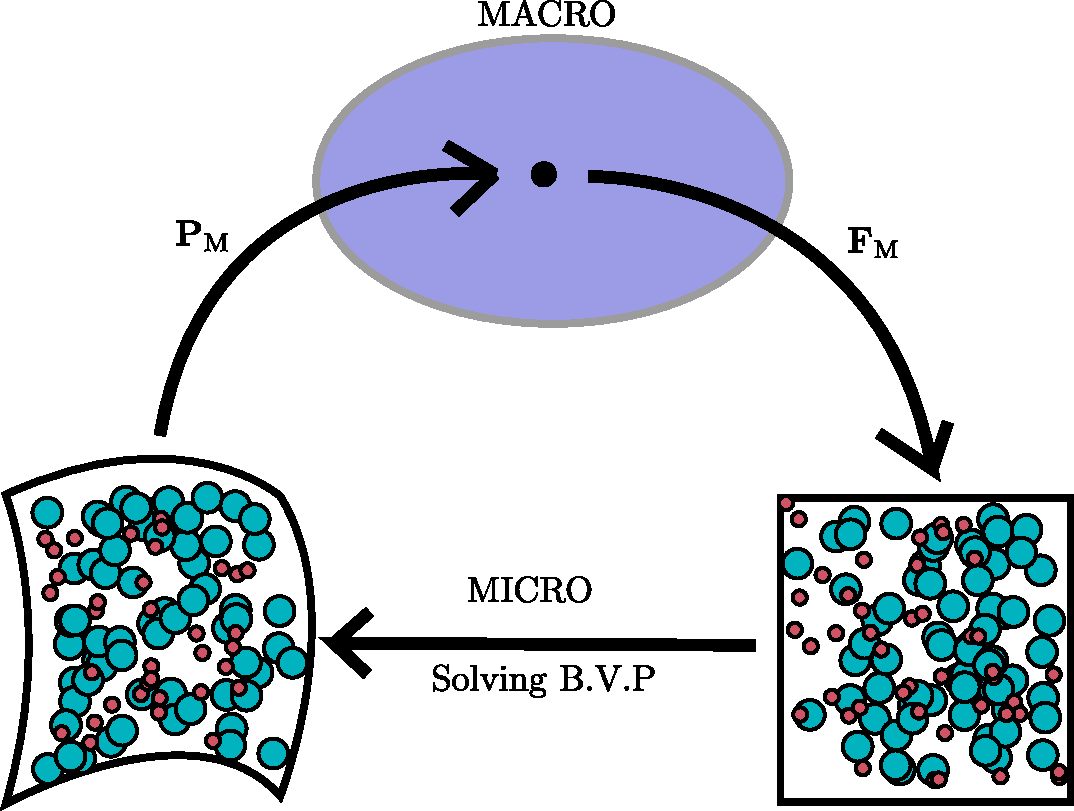
\includegraphics[width=\textwidth]{homogenization_1}
	\end{subfigure}
	\caption{First order computational homogenization of continua.}\label{fig-ch-homogenization}
\end{figure}



This chapter will briefly recall the first order computational homogenization scheme. A periodic boundary condition (PBC) based boundary value problem will be explained that can be used in existing solvers. 
%A self-consistent based homogenization scheme is finally presented that can help avoid boundary effects on RVEs due to the geometrical constraints induced by the RVEs reconstructed from CT-scans of open foam structures, and the reconstruction strategy explained in Chapter \ref{chap-of}. 

The chapter is outlined as follows: In Section \ref{ch-first}, a first order computational homogenization scheme is presented. The corresponding macroscopic formulations, the microscopic formulations and the scale transitions are explained. In Section \ref{ch-periodic}, a PBC based system to solve the boundary value problem presented in Section \ref{ch-first} is explained. In Section \ref{ch-matrices}, the kinematic matrices and their resolution is outlined. 
%Section \ref{ch-self} presents a self consistent homogenization scheme to take into account RVEs that are small in size and for which PBC cannot be directly applied. 

\section{First order computational homogenization}\label{ch-first}

The basic principle of the first order homogenization of mechanical problems is highlighted in Figure \ref{fig-ch-homogenization} where the scale transitions between the two scales are indicated. The deformation gradient, $\textbf{F}_\text{M}$, that constitutes the macroscopic kinematical quantities in this case, is transferred to the micro-scale in order to define a BVP on the RVE. By solving the microscopic BVP in the standard manner, a deformed RVE with corresponding boundary displacements and surface traction is obtained. By making use of standard mathematical averaging equations, the macroscopic stress tensor, $\textbf{P}_\text{M}$, can be extracted. To solve the macroscopic BVP  in parallel, static condensation process can be used to obtain the tangents from the RVE stiffness. This method is also denoted as \fee \cite{feyelFE2MultiscaleApproach2000,feyelMultilevelFiniteElement2003} when the finite element method is used at both scales to solve the entire problem as a nested BVP.

%If we consider the macroscopic nonlinear deformation map, $\mathcal{F}(\tgm[]{X})$, applied to a material vector $\tgm[]{u}$ in the deformed state, then the first order scheme can be written as 
%\begin{equation}
%\tgm[]{u}=\left({\tgm[]{F}-\textbf{I}}\right)\boldsymbol{\cdot}\tgm[]{X}+\tgmm{w}\label{eq-ch-order1}
%\end{equation}
%with $\tgm[]{X}$ and $\tgm[]{X}'$, the associated position vectors in the reference and deformed states respectively, $ \tgm[]{u} $ the reference displacement field and such that $\tgm[]{F}=(\bm\nabla_0\tgm[]{X})^T$. The subscript M represents the macroscopic values. The vector $\tgmm{w}$ represents the micro-fluctuation field that takes into account the local fine scale contribution which is different from the macro-scale deformation\cite{geersMultiscaleComputationalHomogenization2010}. Eq. (\ref{eq-ch-order1}) is valid in every point at the fine scale. In the following subsections, a scale transition from the micro-scale to the macro-scale will be defined to comprehensively link the various stages of computational homogenization.

\red{The separation of scales is an important assumption that can be described as \textit{the microscopic length being much smaller than the characteristic length over which the macroscopic loading varies in space}, i.e.,
\begin{equation}
l_{micro}<<<l_{RVE}<<<l_{macro}
\end{equation}
where $ l_{micro} $ denotes the average size of the pores, inclusions, or grains of the crystals forming the material, $ l_{RVE} $ denotes the size of the RVE and $ l_{macro} $ denotes the characteristic length over which the macro field varies. The condition, $ l_{micro}<<<l_{RVE} $, ensures the statistical representativeness of the micro-scale BVP, while the condition, $ l_{RVE}<<<l_{macro} $, ensures that the average deformation gradient applied on the RVE is meaningful. This also implies that the method is severely limited in the first order case to analyze localization problems since in the latter case $ l_{macro} $ can become smaller than the RVE size, in effect resulting in the loss of the representativeness of the RVE. As a result, the average stress-average strain relationship loses size objectivity beyond strain softening onset. For example, to deal with the problem of failure, other quantities like dissipation energy can be used to characterize the softening homogenized response\cite{nguyenMicromechanicalModelReinforced2019}, or a second order scheme be implemented to handle buckling\cite{nguyenComputationalHomogenizationCellular2014}. However, this second order scheme results in the non-physical problem of persistent gradient effect when the considered RVE is homogeneous, i.e., the response depends on the size of the RVE. A correction, based on micro-structure-dependent body force field can be implemented in the homogenization field along with alternative definitions of localization tensors\cite{yvonnetComputationalSecondorderHomogenization2020,monchietStraingradientHomogenizationBridge2020}. Another class of homogenization, consists of generalized micromorphic continuum that results in an extended continuum at macro-scale by suitable decomposition of the displacement field\cite{rokosExtendedMicromorphicComputational2020,vanbreeNewtonSolverMicromorphic2020}.

However for most of the situations, a first order formulation is sufficient and is a standard tool in computational homogenization\cite{matsuiTwoscaleFiniteElement2004,mcveighMultiresolutionAnalysisMaterial2006,temizerNumericalMethodHomogenization2007,hainComputationalHomogenizationMicrostructural2008}.In this work, we will see that when studying 3D open foam structures in Chapters \ref{chap-of} and \ref{chap-res}, the RVE responses do not exhibit strain softening, justifying the use of the first order homogenization. When considering 2D foam-like structures in Chapter \ref{chap-nn}, a limited softening can be observed before the plateau response, but we consider first order homogenization as an illustration of the data-driven approach, although it should rigorously be extended to a higher order formulation.}

\subsection{Macroscopic formulation}\label{ch-form-macro}
The macro-scale kinematics are defined by the deformation gradient $\tgm[]{F}=\textbf{I}+\tgm[]{u}\otimes\bm\nabla_0$ 
%and its gradient $\tgm[3]{G}=\tgm[]{u}\otimes\bm\nabla_0=\tgm[]{u}\otimes \bm\nabla_0\otimes\bm\nabla_0$
with $ \tgm{u} $ the reference displacement field and $ \bm\nabla_0 $ the gradient operator with respect to the reference configuration. In the absence of body and inertial forces, the strong form of the continuum equilibrium is represented in the body $\Omega$ by
\begin{equation}
	\tgm[]{P}(\tgm[]{X})\cdot\bm\nabla_0
	%-\tgm[3]{Q}(\tgm[]{X}):(\bm\nabla_0\otimes\bm\nabla_0)
	=0,\,\,\,\,\forall\tgm[]{X}\in\Omega.\label{eq-dG-macro}
\end{equation}
where $ \tgm{X} $ is a material point of the body $ \Omega $ expressed in the reference configuration and seen as homogeneous. The boundary conditions read
\begin{subequations}\label{eq-dG-Macro_bc}
	\begin{align}
	\tgm[]{u}(\tgm[]{X}) & =\tgm[]{u}^0, & \forall\tgm[]{X}\in\partial_D\Omega,\\
	\tgm[]{T}(\tgm[]{X}) & =\tgm[]{T}^0, & \forall\tgm[]{X}\in\partial_N\Omega,
%	\text{D}\tgm[]{u}(\tgm[]{X}) & =\text{D}\tgm[]{u}^0, & \forall\tgm[]{X}\in\partial_T\Omega,\\
%	\tgm[3]{R}(\tgm[]{X}) & ={\tgm[3]{R}}^0, & \forall\tgm[]{X}\in\partial_M\Omega,
	\end{align}
\end{subequations}
with constrained displacement $\tgm[]{u}$ on the Dirichlet boundary $ \partial_D\Omega $ and traction per reference unit surface $\tgm[]{T}$ on Neumann boundary $ \partial_N\Omega $
%, and the high order boundary conditions of normal gradient of displacement $\text{D}\tgm[]{u}$ and of double traction per reference unit surface $\tgm[3]{R}$
. Also, 
\begin{equation}\label{eq-DG-bc_exp}
		\tgm[]{T}  = 
		\tgm[]{P}
		\cdot\bar{\mathbf{N}}_\text{M},
\end{equation}
where $\bar{\mathbf{N}}_\text{M}$ is the outward normal in the reference configuration. The stress divergence problem Eq. (\ref{eq-dG-macro}) along with the boundary condition (\ref{eq-dG-Macro_bc}) is completed by the respective constitutive law specifying the stress strain relationships at time $ t $:
\begin{equation}\label{eq-dG-const_macro-1}
	\tgm[]{P}(t) = \mathcal{P}_M\left\{\tgm[]{F}(\tau)
	%,\tgm[3]{G}(\tau)
	,\,\,\tau\in\left[0,t\right]\right\}.
	%\\
	%\tgm[3]{Q}(t) & = \textfrak{Q}\left\{\tgm[]{F}(\tau),\tgm[3]{G}(\tau),\,\,\tau\in\left[0,t\right]\right\}
\end{equation}

The relation (\ref{eq-dG-const_macro-1}) can be represented by introducing the internal state variables $ \tgm[]{Z} $ that denote the representation of the state of the material following the evolution laws of the internal state, with 
\begin{equation}\label{eq-dG-const_macro}
\tgm[]{P}(t) = \mathcal{P}_M\left\{\tgm[]{F}(t),\tgm[]{Z}(t)\right\}.
\end{equation}
The couple $ (\tgm[]{F},\tgm[]{Z}) $ gives a complete description of the constitutive behavior of the state space, and $ \tgm[]{P} $ is an observable quantity. This form of representation can be useful to understand the nature of the material at any given state without having the need to keep the full historical behavior of the material under observation. A general elastic law does not require the use of $ \tgm[]{Z} $.

The weak form corresponding to the system defined by Eqs. (\ref{eq-dG-macro}), (\ref{eq-dG-Macro_bc}) and (\ref{eq-dG-const_macro-1}) can be defined using an admissible kinematic vector field $ \textbf{U}(\Omega) $, where
\begin{equation}\label{eq-dG-law1}
\textbf{U}(\Omega)=\{\delta\tgm{u}\in\mathcal{H}(\Omega)\quad|\quad\delta\tgm{u}|_{\partial_D\Omega}=0\},
\end{equation}
with $ \mathcal{H} $ being the Hilbert space, and the weak form can be summarized as finding $ \tgm{u}\in\mathcal{H}(\Omega) $ such that
\begin{equation}\label{eq-dG-bilinear}
\int_\Omega\left[\tgm{P}(\tgm{u}):\tgm{P}(\delta\tgm{u})\right]\,d\Omega=\int_{\partial_N\omega}\tgm{T}^0\cdot\delta\tgm{u}\,d\partial\Omega\quad\forall\delta\tgm{u}\in\textbf{U}(\Omega)
\end{equation}
with the test function $ \delta\tgm{u} $.

In the context of computational homogenization, the constitutive relationship Eq. (\ref{eq-dG-const_macro}) can be obtained by resolving a microscopic BVP as explained below.

\subsection{Microscopic classical continuum}\label{ch-form-micro}
At the micro scale, the classical continuum assumption is applied. A separation of scale is assumed and the characteristic length of the microscopic BVP is much smaller than that of the continuum scale loading. The BVP is defined on an RVE $ \omega $ of boundary $ \partial\omega $ with the microscopic deformation gradient at a material point $ \tgmm[]{x}\in\omega $ in the reference configuration defined by
\begin{equation}\label{eq-micro-0-1}
\tgmm[]{F}=\textbf{I}+\tgmm[]{u}\otimes\bm\nabla_0,
\end{equation}
where the subscript m represents the local fields of the micro-scale, with the micro-scale reference  displacement field $ \tgmm[]{u} $ and gradient operator $ \bm\nabla_0 $. In the absence of the body sources, the equilibrium state is governed by the following relations,
\begin{equation}\label{eq-micro-1}
\tgmm[]{P}(\tgmm[]{x})\cdot\bm\nabla_0=\bm{0}\,\,\,\,\forall\tgmm[]{x}\in\omega,
\end{equation}
and
\begin{equation}\label{eq-micro-1-1}
\tgmm[]{P}(\tgmm[]{x})\cdot\bar{\mathbf{N}}_\text{m}=\tgmm[]{T}\,\,\,\,\forall\tgmm[]{x}\in\partial\omega,
\end{equation}
with the microscopic first Piola-Kirchhoff stress tensor $ \tgmm[]{P} $, the surface traction per unit surface $ \tgmm[]{T} $ on boundary $ \partial\omega $.
The boundary conditions directly result from the macroscopic variables and the microscopic fluctuations of the displacement field $ \tgmm{w} $ are defined as
\begin{equation}\label{eq-micro-2}
\tgmm[]{w}=\tgmm[]{u}-\left(\tgm[]{F}-\textbf{I}\right)\cdot\tgmm[]{x},
%-\frac{1}{2}{\tgm[3]{G}}:\left(\tgmm[]{x}\otimes\tgmm[]{x}\right)
\end{equation}
which helps achieving the scale transition (Figure \ref{fig-ch-micro}).
\begin{figure}
\centering
\begin{subfigure}[t]{0.75\textwidth}
	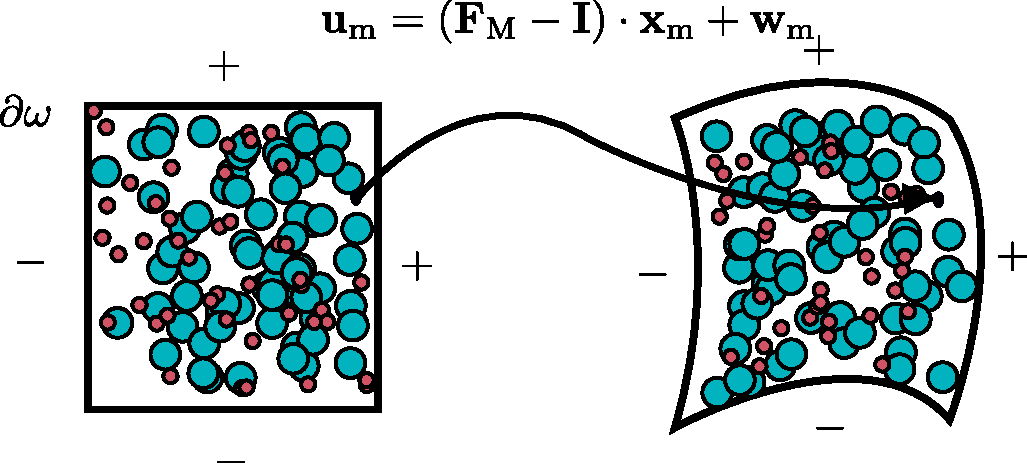
\includegraphics[width=\textwidth]{micro_bvp}
\end{subfigure}
\caption{Deformation of an RVE $ \omega $.}\label{fig-ch-micro}
\end{figure}
The continuum problem (\ref{eq-micro-1}) and its boundary condition (\ref{eq-micro-2}) is completed by a stress-strain relationship defined by a constitutive law at time $ t $
\begin{equation}\label{eq-micro-3-1}
\tgmm[]{P}(t)=\mathcal{P}_m\{\tgmm[]{F}(\tau),\tau\in\left[0,t\right]\}.
\end{equation}
With the introduction of a history-dependent vector $ \tgmm[]{Z} $, Eq. (\ref{eq-micro-3-1}) can be rewritten as
\begin{equation}\label{eq-micro-3}
\tgmm[]{P}(t)=\mathcal{P}_m\{\tgmm[]{F}(t),\tgmm[]{Z}(t)\}.
\end{equation}
In the case of an elasto-plastic material, as it will be used further in this work, this relationship is explicated in Appendix \ref{app-j2} and  \cite{nguyenComputationalHomogenizationCellular2014}.

The weak form corresponding to the system defined by Eqs. (\ref{eq-micro-1}) and (\ref{eq-micro-1-1}) can be defined using a kinematic vector field $ \textbf{U}(\omega)\subset\mathcal{H}(\omega) $, that will be defined during the scale transition.
%\begin{equation}\label{eq-micro-4}
%\textbf{U}(\omega)=\{\delta\tgmm{w}\in\mathcal{H}\left(\omega\right)\quad|\quad\delta\tgmm{w}|_{\partial\omega=0},
%\end{equation}
The weak form can be summarized as finding $ \tgmm{w}\in\textbf{U}(\omega) $ such that
\begin{equation}\label{eq-micro-5}
\int_\omega\tgmm{P}:\left(\delta\tgmm{w}\otimes\bm\nabla_0\right)\,d\omega=\bm{0},\quad\forall\delta\tgmm{w}\in\textbf{U}(\omega),
\end{equation}
with the test function $ \delta\tgmm{w} $.

The analysis of open foam materials involves deformation of individual struts of the RVE which calls for the treatment of surfaces and edges in contact. In this regard, a simple penalty based method has been introduced considering the particular advantage of explicit removal of constraint from the variational formulation leading to an unconstrained optimization\cite{laursenComputationalContactImpact2003}. This problem can be summarized as the addition of $ \Pi^c $ the contact contribution term to the strain energy. Supposing that two surfaces $ \partial\omega_1 $ and $ \partial\omega_2 $ of the body $ \omega $ come into contact, then the value of $ \Pi^c $ can be defined such that
\begin{equation}\label{eq-penalty}
\Pi^c = \frac{1}{2}\int_{\partial_C\omega}\epsilon\,(u_g)^2\,d\partial\omega
\end{equation}
where $ \epsilon>0 $ is the penalty parameter, $  \partial_C\omega $ the domain over which contact action takes place and 
\[ u_g=(\textbf x_2+\textbf{u}_2-\textbf x_1-\textbf{u}_1)\cdot\textbf{n}_1 \ge0\]  
represents the gap between the two surfaces with the unit normal vector $\textbf{n}_1$ defined on the current surface $ \partial\omega_1 $. The master point $ \textbf x_1\in\partial\omega_1 $ is considered as the orthogonal projection of a given slave point $ \textbf x_2\in\partial\omega_2 $ onto the master surface $ \partial_C\omega $ in the deformed configurations characterized by the respective displacements $ \textbf{u}_1 $ and $ \textbf{u}_2 $\cite{wriggersComputationalContactMechanics2006}. The variation of Eq. (\ref{eq-penalty}) gives
\begin{equation}\label{eq-penalty-2}
C_c=\int_{\partial_C\omega}\epsilon\,u_g\,\delta u_g\,d\partial\omega.
\end{equation}
The discretization of the penalty function is explained in detail in \cite{wriggersComputationalContactMechanics2006}.

\subsection{Scale transition}\label{ch-form-scale}

The scale transition can be complemented by two averaging equations:
\begin{enumerate}
	\item volume averaging of the deformation $\textbf F_\text M$ or stress $\textbf P_\text M$, defined as
	\begin{equation}\label{eq-st-1}
	\tgm[]{F}=\frac{1}{\omega}\int_\omega\tgmm[]{F}d\omega,
	\end{equation}
	and,
	\begin{equation}\label{eq-st-2}
	\tgm[]{P}=\frac{1}{\omega}\int_\omega\tgmm[]{P}d\omega;
	\end{equation}
	\item the Hill-Mandel macro-homogeneity condition, or the volume averaging of the virtual work, defined as
	\begin{equation}\label{eq-st-3}
	\tgm[]{P}:\delta\tgm[]{F}
	%+{\tgm[3]{Q}}:\delta{\tgm[3]{G}}
	=\frac{1}{\omega}\int_\omega\tgmm[]{P}:\delta\tgmm[]{F}d\omega,
	\end{equation}
	that ensures that the sub-scale modeling is energetically consistent.
\end{enumerate}

%and
%\begin{equation}\label{eq-st-3}
%\tgm[3]{q}=\frac{1}{2\omega}\int_\omega\tgmm[]{P}\otimes\tgmm[]{x}+\left(\tgmm[]{P}\otimes\tgmm[]{x}\right)^{RC}d\omega,
%\end{equation}
%where for any third order tensor $ ^3\textbf{A} $, $ A^{RC}_{ijk}=A_{ikj} $.
The homogenized stress also gives the first order tangent $ \tgm[]{L} $
%and the second order tangent $ \tgm[3]{J} $ 
as
\begin{eqnarray}\label{eq-st-4}
\tgm[]{L}=\frac{\partial\tgm[]{P}}{\partial\tgm[]{F}}. 
\end{eqnarray}

To ensure that the Hill-Mandel principle is \textit{a priori} satisfied, the boundary condition applied on the micro-scale BVP must be analyzed appropriately.

Using Gauss theorem on Eq. (\ref{eq-micro-2}), a constraint on the fluctuation field in the following form can be introduced using Eq. (\ref{eq-st-1}):
\begin{equation}\label{eq-st-5}
\int_{\partial\omega}\tgmm{w}\otimes\bar{\textbf{N}}_\text{m}\,d\partial\omega=\int_\omega\tgmm{w}\otimes\bm\nabla_0\,d\omega=\bm{0}.
\end{equation}
The Hill-Mandel principle Eq. (\ref{eq-st-3}) can be rewritten using Eq. (\ref{eq-micro-2}) in the following form:
\begin{eqnarray}\label{eq-st-6}
\tgm{P}:\delta\tgm{F} & = & \frac{1}{\omega}\int_\omega\tgmm{P}:\delta\tgmm{F}\,d\omega\nonumber\\
& = & \tgm{P}:\delta\tgm{F}+\frac{1}{\omega}\int_\omega\tgmm{P}:\left(\delta\tgmm{w}\otimes\bm\nabla_0\right)\,d\omega.
\end{eqnarray}
By using integration by parts on Eq. (\ref{eq-st-6}) and on the basis of equilibrium equations stated in Eqs. (\ref{eq-micro-1}-\ref{eq-micro-1-1}), one has
\begin{equation}\label{eq-st-7}
\int_{\partial\omega}\left(\tgmm{P}\cdot\bar{\textbf{N}}_\text{m}\right)\cdot\delta\tgmm{w}\,d\partial\omega=\int_{\partial\omega}\tgmm{T}\cdot\delta\tgmm{w}\,d\partial\omega=\bm{0}.
\end{equation}
The minimum kinematic vector field $ \textbf{U}^{\min}(\omega) $ is defined by Eq. (\ref{eq-st-5}). Indeed, the solution $ \tgmm{w}\in\textbf{U}^{\min}(\omega) $ that satisfies Eq. (\ref{eq-micro-5}) for all $ \delta\tgmm{w}\in\textbf{U}^{\min}(\omega) $ automatically satisfies the Hill-Mandel condition (\ref{eq-st-6}) and thus (\ref{eq-st-7}). However, stronger kinematic field $ \textbf{U}(\omega)\subset\textbf{U}^{\min}(\omega) $ are usually considered as the PBC.

\section{Micro-scale boundary conditions}\label{ch-periodic}

The BVP can be expressed through prescribed displacement $\tgmm{u}^*$ of some characteristic boundary points of the RVE as,
\begin{equation}
\tgmm{u}^*=\textbf{f}(\tgmm[]{x},\tgm{F}).\label{eq-ch-bc}
\end{equation}
It can be seen from Eq. (\ref{eq-ch-bc}) that the macroscopic deformation enters the micro-scale BVP through the boundary conditions of the RVE. These boundary conditions result from the adopted micro-macro averaging relations. Traditionally, one can apply a uniform traction field in what is known as constant traction boundary condition (or Neumann BC) on the RVE boundary $ \partial\omega $ prescribed in terms of macroscopic stress as
\begin{equation}\label{eq-periodic-0-1}
\tgmm{T}=\tgm{P}(\tgmm{x})\cdot\bar{\textbf{N}}_\text{m}\quad\forall\tgmm{x}\in\partial\omega,
\end{equation}
or a displacement field in what is known as linear displacement boundary condition (Dirichlet BC) on the RVE boundary $ \partial\omega $ constrained in terms of macroscopic strain as
\begin{equation}\label{eq-periodic-0-2}
\tgmm{w}=\tgmm{u}-(\tgm{F}-\textbf{I})\cdot\tgmm{x}=0\quad\forall\tgmm{x}\in\partial\omega
\end{equation}
Both the conditions satisfy Eq. (\ref{eq-st-7}), and in the context of kinematic finite element, the condition (\ref{eq-periodic-0-2}) satisfies Eq (\ref{eq-st-5}) and can be directly applied for a given $ \tgm{F} $. However, the condition (\ref{eq-periodic-0-1}) is known to be too compliant while the condition (\ref{eq-periodic-0-2}) is too stiff. Periodic boundary conditions are one of the most versatile boundary conditions that can be used for both periodic and non-periodic underlying micro-structures\cite{kouznetsovaApproachMicromacroModeling2001,mieheStraindrivenHomogenizationInelastic2002}. 
%Some other boundary conditions include Kinematic Uniform Boundary Conditions (KUBC), Zero Average Fluctuation Boundary Condition (ZAFBC), and Static Uniform Boundary Condition (SUBC)\cite{nguyenUnifiedTreatmentMicroscopic2017}.

The efficiency of periodic boundary conditions in case of conformal meshes makes it an ideal candidate to be used in the BVP considered along with its ability to provide a better estimation in comparison with Dirichlet or Neumann conditions\cite{nguyenImposingPeriodicBoundary2012}. 

The periodicity of the fluctuation field in Eq. (\ref{eq-micro-2}) can be constrained by
\begin{eqnarray}\label{eq-periodic-2}
\begin{array}{l l l l}
\tgmm[]{w}(\tgmm[]{x}^+)=\tgmm[]{w}(\tgmm[]{x}^-) & \forall\tgmm[]{x}^-\in\partial\omega^- & \text{and matching} & \tgmm[]{x}^+\in\partial\omega^+.
\end{array}
\end{eqnarray}
%and
%\begin{equation}\label{eq-periodic-0-3}
%\int_{\partial\omega_{Pi}}\tgmm{w}(\tgmm{u})\,d\partial\omega=\bm{0}\quad \forall\partial\omega_{P}\subset\partial\omega^-,
%\end{equation}
with $ \partial\omega^- $ and $ \partial\omega^+ $ being the negative and positive parts of the boundary $ \partial\omega $, such that
\begin{equation}\label{eq-perioidic-3}
\partial\omega^-\cup\partial\omega^+=\partial\omega,
\end{equation}
and
\begin{equation}\label{eq-perioidic-4}
\partial\omega^-\cap\partial\omega^+=\emptyset.
\end{equation}.
%$ \partial\omega_{Pi} $ with $ i\in\mathcal{N}_{elements} $ and $ \partial\omega_P $ representing the boundary elements on $ \partial\omega^- $.

\begin{figure}
	\centering
	\begin{subfigure}[t]{0.5\textwidth}
		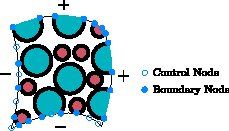
\includegraphics[width=\textwidth]{ch-periodic}
	\end{subfigure}
	\caption{Depiction of the boundary and control nodes on an non-periodic RVE to implement polynomial interpolation method.}\label{fig-ch-periodic}
\end{figure}

The constraints imposed on the matching nodes of a periodic micro-structure makes the implementation straightforward. However in the case of non-periodic underlying geometry, a polynomial interpolation-based approach as explained in \cite{nguyenImposingPeriodicBoundary2012,nguyenComputationalHomogenizationCellular2014} is more suitable for RVEs with dominant presence of voids on the boundary. This approach is briefly summarized here. 

To enforce this constraint on a non-periodic mesh with the presence of void parts on the RVE boundary, the perturbation field needs to be interpolated on the negative and positive parts of the RVE boundary with a defined interpolant function using a set of control nodes (Figure \ref{fig-ch-periodic}). With the help of interpolant functions $ \mathbb{N}^k(\tgmm[]{x}) $, Eq. (\ref{eq-periodic-2}) 
%and \ref{eq-periodic-3} 
can be written as
\begin{equation}\label{eq-periodic-3}
\tgmm[]{w}^-(\tgmm[]{x})  = \underset{k}{\sum}\mathbb{N}^k(\tgmm[]{x})\tgmm[]{w}^k,
\end{equation}
\begin{equation}\label{eq-periodic-3-1}
\tgmm[]{w}^+(\tgmm[]{x})  = \underset{k}{\sum}\mathbb{N}^k(\tgmm[]{x})\tgmm[]{w}^k,
\end{equation}
and
\begin{equation}\label{eq-periodic-4}
\int_{\partial\omega^-}\left(\sum_k\mathbb{N}^k(\tgmm{x})\tgmm{w}^k\right)\,d\partial\omega=\bm{0}.
\end{equation}
with the fluctuation terms $ \tgmm{w}^k $ at the control node $ k $.
The interpolant function chosen defines the choice of $ \tgmm[]{w}^k $. By recalling the fluctuation term defined in Eq. (\ref{eq-micro-2}), the system of Eqs. (\ref{eq-periodic-3}), (\ref{eq-periodic-3-1}) and (\ref{eq-periodic-4}) can be written as,
\begin{equation}\label{eq-periodic-5}
\tgmm{u}^-(\tgmm{x})-\sum_k\mathbb{N}^k(\tgmm{x})\tgmm{u}^k=\left(\tgm{F}-\textbf{I}\right)\cdot\left[\tgmm{x}-\sum_k\mathbb{N}^k(\tgmm{x})\tgmm{x}^k\right],
\end{equation}
\begin{equation}\label{eq-periodic-5-1}
\tgmm{u}^+(\tgmm{x})-\sum_k\mathbb{N}^k(\tgmm{x})\tgmm{u}^k=\left(\tgm{F}-\textbf{I}\right)\cdot\left[\tgmm{x}-\sum_k\mathbb{N}^k(\tgmm{x})\tgmm{x}^k\right],
\end{equation}
and
\begin{equation}\label{eq-periodic-5-2}
\int_{\partial\omega^-}\left(\sum_k\mathbb{N}^k(\tgmm{x})\tgmm{u}^k\right)d\partial\omega=\left(\tgm{F}-\textbf{I}\right)\cdot\left[\int_{\partial\omega^-}\sum_k\mathbb{N}^k(\tgmm{x})\tgmm{x}^k\,d\partial\omega\right].
\end{equation}

The control nodes introduce additional degrees of freedom in the system. A detailed study on the types of interpolation formulations has been presented in \cite{nguyenImposingPeriodicBoundary2012} ranging from Lagrange interpolation and B-splines in the case of 2D and surface B-splines and bi-linear patch Coons formulations in the case of 3D. A finite element based formulation can also be considered to implement periodicity in boundary condition on non-conformal meshes, inducing a quasi-periodic boundary condition\cite{wismansComputedTomographybasedModeling2009}.

\section{Kinematic matrices and resolution}\label{ch-matrices}
After finite element discretization, the macroscopic weak form Eq. (\ref{eq-dG-bilinear}) can be written as 
\begin{equation}\label{eq-res-1}
{\tgm[]{f}}_{\text{int}}(\tgm[]{u})-\tgm[]{q}=\bm{0},
\end{equation}
with the internal force $  {\tgm[]{f}}_{\text{int}}(\tgm[]{u}) $ computed from the bulk and surface integrals and $ \tgm[]{q} $ equivalent to the linear form $ b(\tgm[]{u}) $.

The microscopic weak form  (\ref{eq-micro-5}) along with the system of boundary conditions (\ref{eq-periodic-5}), (\ref{eq-periodic-5-1}) and (\ref{eq-periodic-5-2}) can be represented in the non-linear form
\begin{eqnarray}\label{eq-res-2}
\tgmm[]{f}(\tgmm[]{u})-\textbf{C}^T\lambda=\bm{0}\nonumber\\
\textbf{C}\textbf{u}_b-\textbf{g}=\bm{0}
\end{eqnarray}
with the constraints coefficients matrix $ \textbf{C} $, a regrouped unique vector that combines the degrees of freedom of the boundary and control nodes $ \textbf{u}_b $ and the loading part $ \textbf{g}=\textbf{g}(\tgm[]{F}) $ that depends only on the macroscopic strains for a given RVE.

The resolution of this constrained micro-scale BVP can be achieved using the multiplier elimination approach\cite{ainsworthEssentialBoundaryConditions2001}. This method allows the treatment with a unified multiple constraint and has been found successful to enforce microscopic boundary condition. A path following based strategy combined with arc-length increment constraint can be successfully integrated with the multiplier elimination approach to skip through the critical points and unstable equilibrium paths involved in the non-linear response, thus ensuring the convergence of the Newton-Raphson strategy. This combination is explained in detail in \cite{nguyenComputationalHomogenizationCellular2014,nguyenUnifiedTreatmentMicroscopic2017}. The finite element method to solve the macro-scale BVP is briefly recalled in Appendix \ref{app-fem}.

%\section{Self-consistent homogenization}\label{ch-self}
%In the following chapters, discussions pertaining to extraction and reconstruction of specific open foam morphologies from physical samples based on CT-scan and image processing will be presented. A recurrent problem in these kinds of extracted models is that these small sized RVEs constrain the ability of the previously described PBC based interpolations to obtain an effective homogenized properties. Due to the limited size of the RVE, the boundary conditions bring in constraints that prevent the buckling of the incomplete struts on the boundaries. This calls for approaches that expand the domain by introducing material that mimic the behavior of the RVE without actually influencing the RVE.
%
%An approach to overcome such problems using a volumetric coupling is described in \cite{cottereauStochasticdeterministicCouplingMethod2013}. In this method, originally developed to account for the loss of statistical representability of a too small RVE, a stochastic volume element (VE) is coupled to an embedding deterministic domain by expanding the Arlequin coupling method\cite{dhiaArlequinMethodFlexible2005}. The method essentially is an optimization problem that necessitates an estimation of the homogenized tensor to be applied on the embedding deterministic domain through a fixed point iterative scheme. The idea is that the optimized homogenized model will on average behave exactly the same way whether they are solved alone or coupled with the micro-structure. In other words, the solution of the homogenized model and the model coupled with the micro-structure should be the same on average. Any general purpose optimization scheme can be used to solve for the optimization problem, like the Nelder-Mead algorithm\cite{gaoImplementingNelderMeadSimplex2012}. In this work, we are not interested by the stochastic nature of the VE, but as previously explained, aim at representing the exact behavior for the external struts.
%
%\begin{figure}
%	\centering
%	\begin{subfigure}{0.5\textwidth}
%		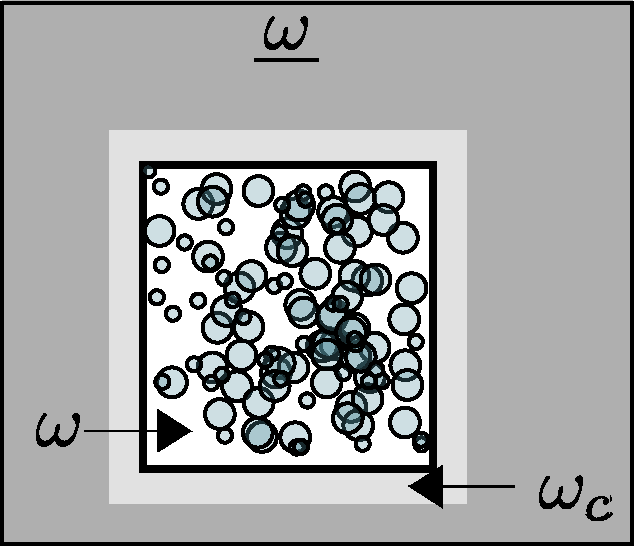
\includegraphics[width=\textwidth]{stochastic_self}
%		\caption{}
%	\end{subfigure}
%	\begin{subfigure}{0.39\textwidth}
%		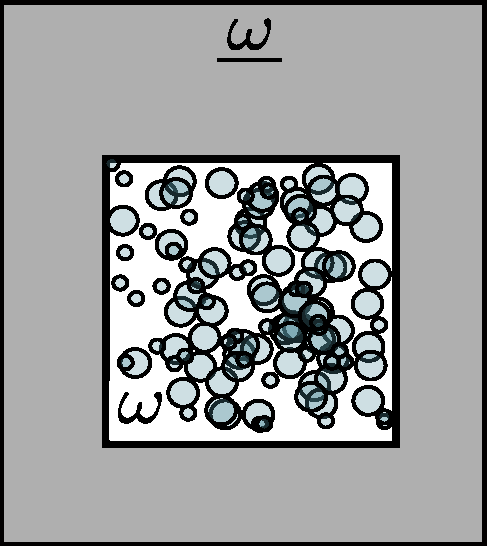
\includegraphics[width=\textwidth]{stochastic_self_no_couple}
%		\caption{}
%	\end{subfigure}
%	\caption{Self-consistent homogenization; (a) An Arlequin problem in 2D defined over the domain $\underline{\omega}$ by the effective model, over domain $ \omega $ by the random model RVE, and coupled over the domain $ \omega_c $, as explained in \cite{cottereauStochasticdeterministicCouplingMethod2011}; (b) Simplified deterministic embedding domain $\underline{\omega}$ around the RVE $ \omega $.}\label{fig-ch-self}
%\end{figure}
%
%Consider that the RVE micro-structure is defined over domain $ \omega $, with a parameter field $ \textbf{k} $. The embedding effective model is then defined over the domain $ \underline{\omega} $ defined by an appropriate material law representing the homogenized behavior and a set of constant parameters $ \underline{\textbf{K}} $. The two domains are defined such that $ \omega\subset\underline{\omega} $ and their intersection over which the two domains communicate is $ \omega_c $ (Figure \ref{fig-ch-self}a). This necessarily means that there is some part of the domain where only the deterministic effective model applies, some part of the domain were the coupling occurs and where both the models are defined, and finally the part where both the models are defined but do not communicate. The alternative used in this work is illustrated in Figure \ref{fig-ch-self}b in which a strong coupling is considered between $ \omega $ and $ \underline{\omega} $.
%
%By taking inspiration from this method, one can introduce a self-consistent homogenization scheme that presents a systematic procedure to determine the non-physical deterministic material law parameters. In this work the fine-scale parameter will be taken to be an elasto-plastic material as described in Appendix \ref{app-j2}. The model of the embedding domain can be chosen as a polynomial model described in Appendix \ref{app-hyper} or a non-visous plasticity model. The optimization problem of the self-consistent scheme can be summarized as follows
%\begin{enumerate}
%	\item Using simple assumptions derived from the RVE model parameter $ \textbf{k} $ on $ \omega $, initialize the parameters $ \underline{\textbf{K}} $ of the effective model on $ \underline{\omega} $ to $ \underline{\textbf{K}}^0 $. 
%	\item\label{list-homo-1} Solve the coupled BVP on $ \omega+\underline{\omega} $ by applying PBC on $ \underline{\omega} $ in order to obtain necessary indicators like nodal displacements $ \tgmm{w} $ of the RVE $ \omega $.
%	\item\label{list-homo-2} Compare the homogenized response of $ \omega $ and of the coupled problem $ \omega+\underline{\omega} $.
%	\item\label{list-homo-3} Using an optimization algorithm based on Nelder-Mead methods, or similar methods (like the \textit{fminsearch} function in MATLAB\textregistered), optimize the material parameters $ \underline{\textbf{K}} $ to $ \underline{\textbf{K}}^i $ by comparing the recorded indicators in Step \ref{list-homo-2}, so as to minimize their difference. Since resolution of the coupled problem $ \underline{\omega}+\omega $ is time consuming due to the complexity of $ \omega $, the optimization algorithm is modified as follows:
%	\begin{enumerate}
%		\item Replace the micro-structure $ \omega $ by a homogeneous medium $ \overline\omega $ with properties $ \overline{\textbf{K}} $ initialized to $ \underline{\textbf{K}}^{i-1} $.
%		\item Iterate on $ \overline{\textbf{K}} $ so that the stress-strain curve of $ \overline\omega $ match the stress strain curve of $ \underline{\omega} $.
%		\item Once converged, use $ \overline{\textbf{K}} $ as the new embedding properties $ \underline{\textbf{K}}^i $.
%	\end{enumerate}
%	\item Repeat steps \ref{list-homo-1} to \ref{list-homo-3} until the tolerance criterion $ \epsilon $ is reached, such that $ ||\underline{\textbf{K}}^{i+1}-\underline{\textbf{K}}^i||<\epsilon $.
%\end{enumerate}
%Figure \ref{fig-self-consistent} summarizes the above algorithm for a uniaxial compression loading.
%\begin{figure}
%	\centering
%	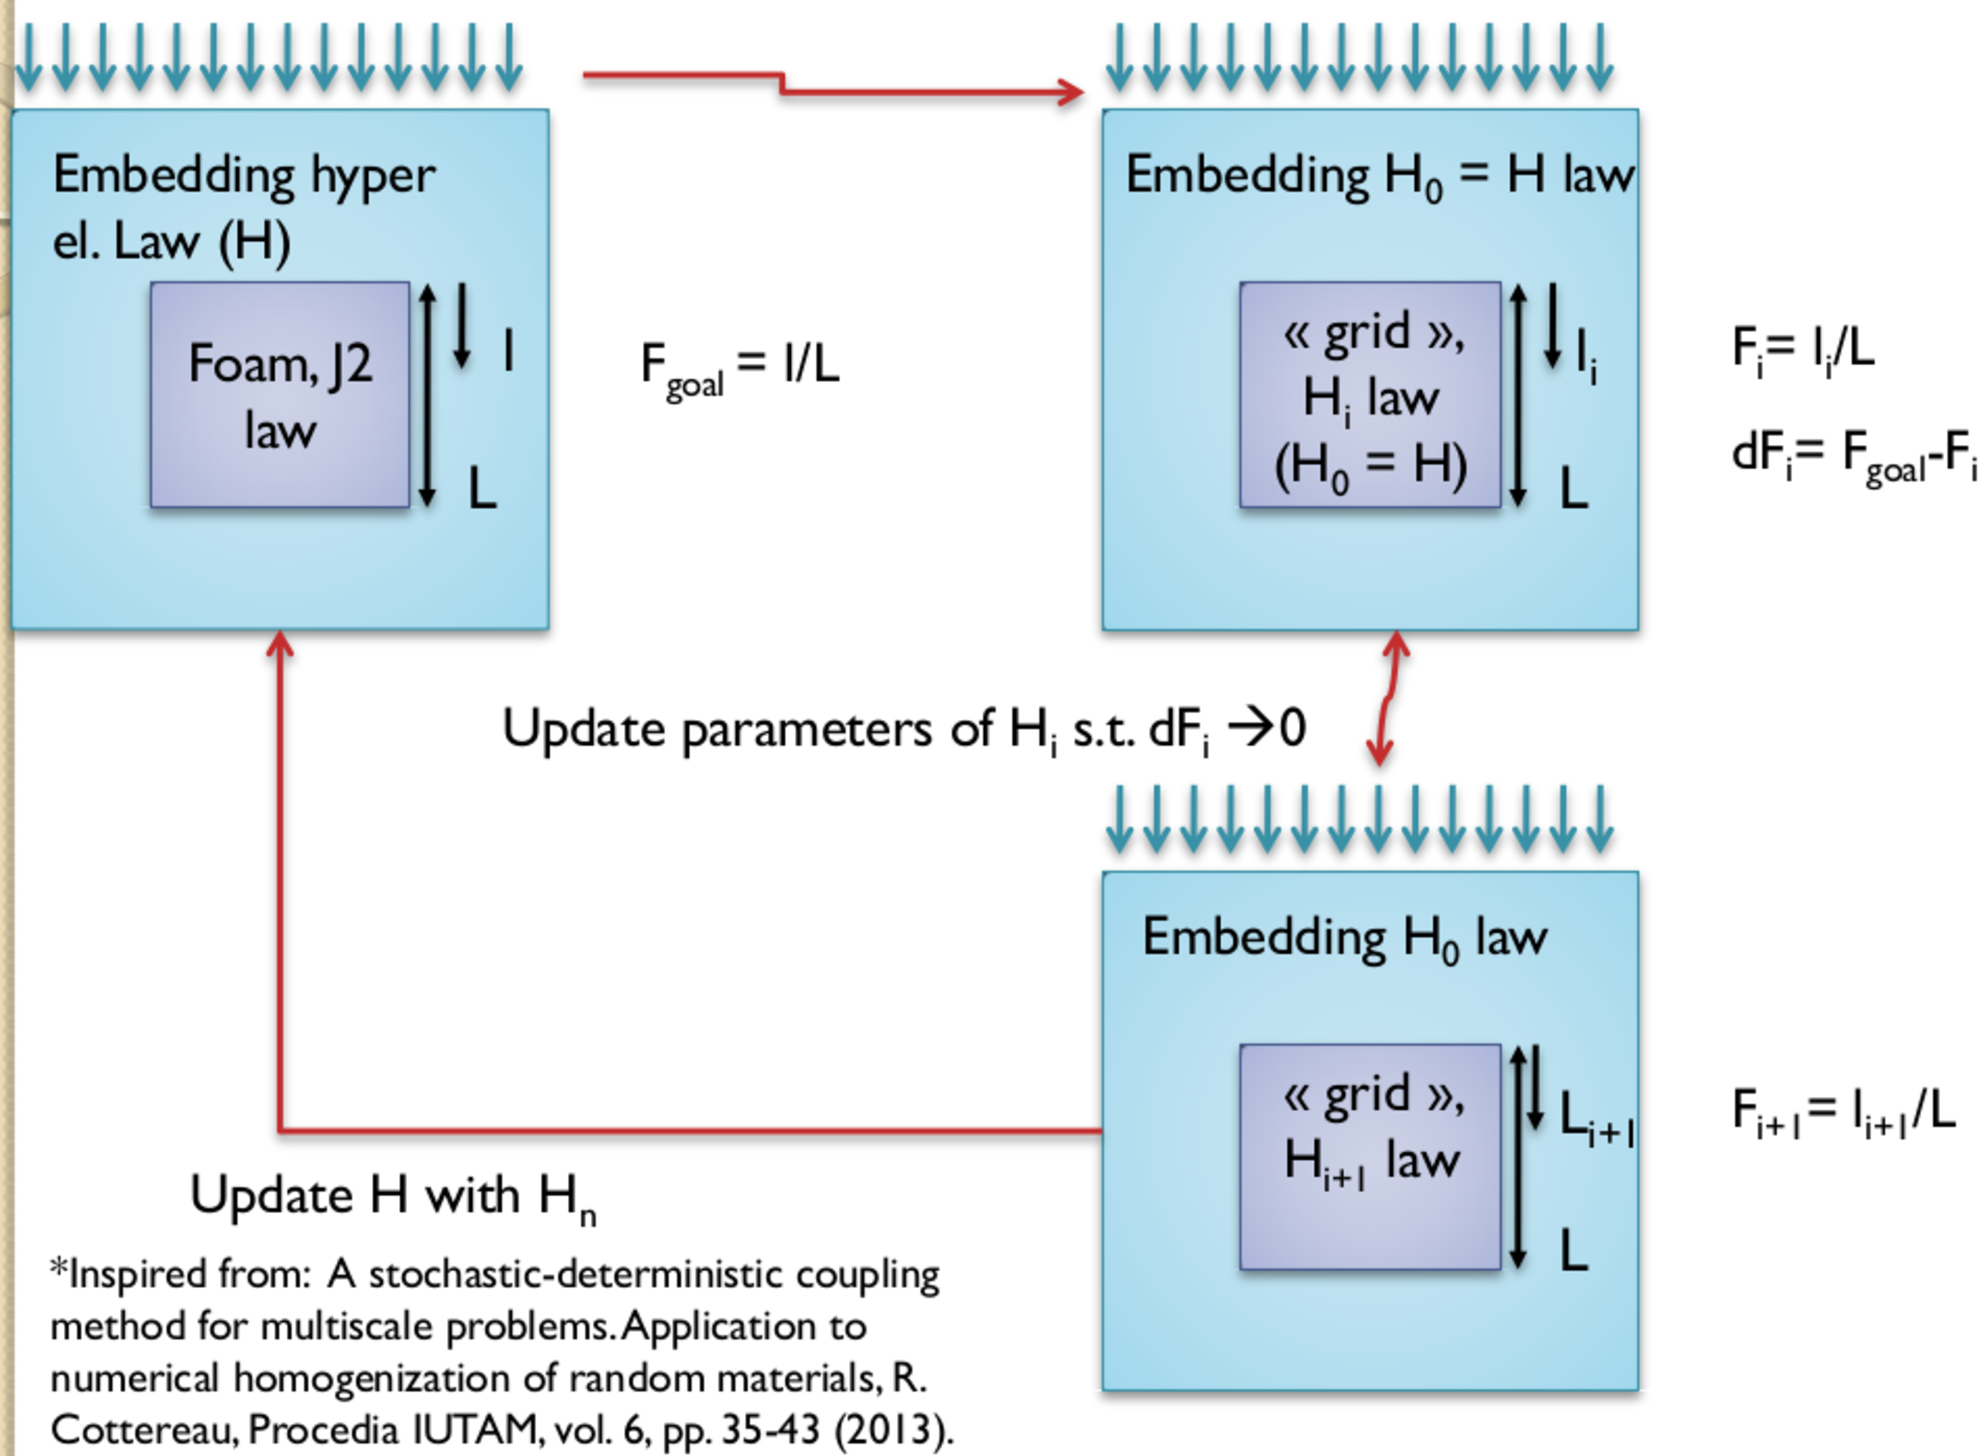
\includegraphics[width=\textwidth]{self_consistent}
%	\caption{Reference figure (TO REDRAW according to text); Modified self consistent scheme for a uniaxial compression test where the optimization is done by replacing the complex micro-structure with a simpler geometry to reduce computational time\cite{leblancAnalysisOpenFoamUnderPreparation}.}\label{fig-self-consistent}
%\end{figure}

\section{Conclusions}
The computational homogenization theory has been recalled in this chapter to effectively resolve a micro-macro based finite element problem. In order to be energetically consistent, suitable formulations for the microscopic and macroscopic continuum problem have been presented along with the necessary relations to perform an efficient scale transition. A periodic boundary condition based system has been presented that ensures that the energy conservation principle is satisfied while undergoing scale transition. 
%To aid in the homogenization process, in the case of smaller RVEs, a self consistent homogenization procedure has also been outlined.

To solve this \fee computational homogenization, a suitable RVE that represents the micro-structure of the chosen heterogeneous material needs to be discretized into finite elements. In Chapter \ref{chap-of}, a micro-structure generation tool is presented to extract open foam morphologies with particular attention paid to the strut geometries. The procedure to discretize the open foam geometry into finite elements will also be detailed. To ensure that the RVE is truly representative, the geometry needs to be statistically representative of all the microscopic properties of the open foam. Chapter \ref{chap-res} compares the geometries extracted to ensure that a given RVE is truly representative. 

The resolution of the system of equations for computational homogenization method outlined in Eqs. (\ref{eq-res-1}) and (\ref{eq-res-2}) is an iterative process that needs to be carried out at each integration point of the macro-scale finite element. This is the most computationally expensive process of the \fee method as it has to be repeated for each macro-scale iteration. Chapter \ref{chap-nn} details some data-driven surrogate models that can be adopted to replace this step and reduce the computational expense.